\chapter{Overview}
\label{chap:overview}
% - Overview - problem description - introduce tool - outline thesis
\section{Problem Description}

Command line interfaces have been with us since the 1950s
\cite{raymond2004art}. The rise of command line interfaces was closely coupled
with the rise of time-sharing computer systems. Command line interfaces and
time-sharing systems greatly shortened the feedback loop of earlier batch
computing systems and allowed programmers to be able to modify their programs
in near real time. Time-sharing systems also introduced the concept of a
\textit{shell}. A \textit{shell}, a term coined by Louis Pouzin \cite{pouzin},
is a program that allows for interaction with the operating system via textual
commands\cite{mashey1976using}. The \textit{Multics}\cite{corbato1965introduction} operating system
pioneered the concept of operating system shells. The concept proved to be
extremely influential and directly influenced the creation of the
\textit{Thompson shell} for the \textit{UNIX} \cite{ritchie1974unix} operating
system. The \textit{UNIX} shell has arguably had the greatest influence on
command line interfaces as we know them today, as most modern shells are
descendants of the original \textit{UNIX} shell \cite{raymond2004art}.

The command line is still a popular interaction medium for tooling in the areas
of software engineering and system administration
\cite{hultstrand2015git, takayama2006trust}. However, the usage of the command
line in the general personal computing space has practically disappeared
\cite{reimer2005history}. This is especially true for younger individuals,
whose very first exposure to computers has been working with Graphical User
Interfaces (GUIs). This schism in interaction mediums causes issues when the
same younger individuals strive to enter technical fields such as software
development or system administration. The issue is further propagated by the
fact that the command line is its own distinct interaction paradigm based
entirely on writing and reading text. This can mean that the usage of
traditional learning resources such as documentation and manuals might prove
difficult to translate into effective usage without active textual interaction
practice on the part of the learner. On the other hand, jumping straight into
practising on the command line comes with its caveats. The shell can be an
unforgiving tool for a novice user as it is very sensitive to syntax and often
provides feedback that is difficult to understand for novice users. The shell
also interacts directly with the operating system and does not require
confirmation for certain destructive tasks such as file deletion.

\subsection{Solving The Problem} The goal of this Master's thesis is to develop
a tool that simultaneously aims to address the previously introduced issues of
lack of exposure to textual interaction, the novice unfriendly environment of
the shell and the difficulties of traditional learning methodologies. The tool
should provide a more forgiving experience than using the shell directly whilst
still being a faithful representation of a system shell. Concepts learned
during the interactive tutorials should be directly transferrable to a standard
Unix-like shell. Furthermore, the tool should be easy to use and encourage
experimentation in order to augment the learning experience and in order to
better exploit the advantages offered by interactive learning systems.
%TODO: Expand a bit

% \fig[0.75\textwidth]{img/vimtutor}{Screenshot of vimtutor}{fig:vimtutor}
\section{Introducing "CLI-Tutor"}
\begin{figure}[htbp]
	\centering
	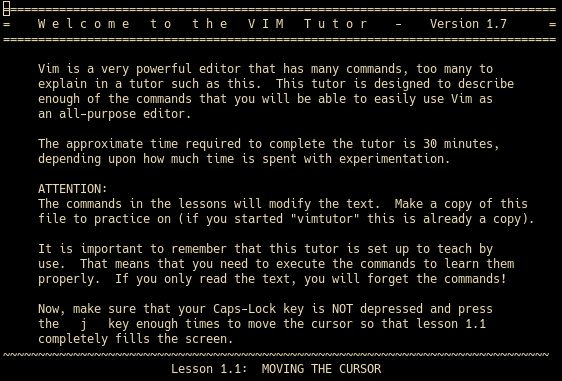
\includegraphics[width=0.75\textwidth]{img/vimtutor}
	\caption{Screenshot of \textit{vimtutor}}
	\label{fig:vimtutor}
\end{figure}

The \textit{CLI-Tutor} tool is an interactive shell-like tutorial program for
the command line. We draw inspiration from the
\textit{vimtutor}\cite{pierce_ware_smith_moolenaar_2019} (see: Figure
\ref{fig:vimtutor}) utility shipping alongside the popular terminal-based text
editor \textit{Vim}. \textit{Vimtutor} is an interactive tutorial for the Vim text
editor. It is one long guided lesson presented as a text file. The file itself
contains the basic instructions for editing and creating text within Vim and is
intended to be modified while proceeding through the lesson. This "learning by
doing" approach presented itself as a very suitable choice for teaching the
command line. Much like with Vim, where one must learn a new paradigm of modal
editing when novices learn the command line they are not only taking on new
information about shell usage but also learning an entirely unfamiliar
(textual) interaction paradigm. Newer versions of \textit{vimtutor} are even more
interactive. In the version included in the popular fork of Vim called \textit{Neovim}
\cite{neovimHomeNeovim}, lines intended to be edited by the user also provide
feedback regarding correctness in the form of green arrows and red crosses.

The \textit{CLI-Tutor} tool introduces users to topics such as shell basics and
Unix-like core utility usage through a series of interactive examples. The tool
aims to relax the steep learning curve associated with the command line by
leveraging interactive examples and a feedback mechanism to instruct and
educate the user about the current stage of the lesson and provide some
feedback based on the inputs of the user. The core of \textit{CLI-Tutor} is
contained within a command line application written in golang\footnote{Go
	programming language: \href{https://go.dev/}{https://go.dev/}} and serves as a
standalone application. However, in order to make the learning experience safer
for the user and to encourage exploration, the CLI application has been wrapped
into a web application to form a sandboxed environment for the user that
exposes a terminal over the web. This means the user can use the tutorial
application without fear of causing their own system any harm.

The \textit{CLI-Tutor} application is fully open source and also comes with its
own modified parser and structure for specifying lessons based on Markdown
documents. This means that the material covered by the lessons can be easily
contributed to and distributed, making the tool easily extensible.


% \fig[0.75\textwidth]{img/clitutor}{Screenshot of CLI-Tutor}{fig:clitutor}
% \begin{figure}[htbp]
\begin{figure}[H]
	\centering
	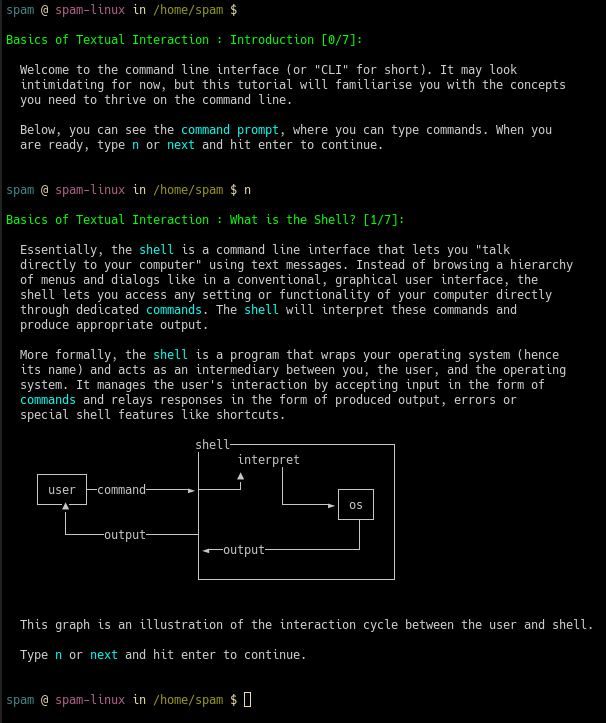
\includegraphics[width=0.75\textwidth]{img/clitutor}
	\caption{Screenshot of \textit{CLI-Tutor}}
	\label{fig:clitutor}
\end{figure}

\section{Thesis Outline}

Over the next few chapters, we will discuss and show the design, implementation
and overall goals of this solution. \autoref{chap:intro} will discuss the
problem space and explain the motivations behind the interactive approach
employed by \textit{CLI-Tutor}. In \autoref{chap:clitutor}, the semantic
aspects CLI application and associated web application will be discussed. We
will discuss the design and implementation of the solution in
\autoref{chap:design}. \autoref{chap:userstudy} will discuss the methodology
and findings of the user study conducted during this Master's thesis work. In
\autoref{chap:reflection}, we will evaluate and reflect upon the solution. We
will consider existing approaches and make suggestions regarding building upon
and refining the \textit{CLI-Tutor}, before, concluding in
\autoref{chap:conclusion}.


